\chapter{کار‌های مشابه}
\section{مقدمه}
در این فصل هدف ما بررسی پروژه های مشابه است تا بتوان از آنها در روند پروژه کمک گرفت. همچنین در این راه می‌توان با توجه به نتایج و ارزیابی پروژه‌های دیگر بستری را فراهم کرد تا نتیجه پروژه را با دیگر کارهای مشابه مقایسه کرد.
\\
به صورت کلی پروژه‌هایی با هدف کنترل پهپاد با ژست دست در 2 دسته قرار می‌گیرند.
\begin{itemize}
    \item کنترل پهپاد با کمک بینایی ماشین که شامل شبکه‌هایی برای پردازش تصویر است. 
    \item کنترل پهپاد با دستکش‌های سنسور دار از جمله سنسور \lr{IMU} که نیازمند سخت‌افزار خاص برای پیدا کردن موقعیت نقاط دست است. مانند پروژه‌های \lr{Motion Estimation and Hand Gesture Recognition-Based Human–UAV Interaction Approach in Real Time} \cite{yoo2022motion} و \lr{Hand gesture recognition with convolutional neural networks for the multimodal UAV control} \cite{ma2017hand}.
    \item وجود دستگاه کنترل کننده حرکت جهشی\lr{Leap Motion Controller} که با توجه آن ویژگی‌های دست با دقت بالا اندازه گیری شده و با کمک شبکه‌های عصبی ژست دست تشخیص داده میشود. پروژه‌ی
    \lr{Deep Learning Based Hand Gesture Recognition and UAV Flight Controls} \cite{hu2020deep} و \lr{Gesture control of drone using a motion controller} \cite{sarkar2016gesture} نمونه‌ای از این جمله پروژه‌ها هستند. 
\end{itemize}

از بین این موارد پروژه ما مربوط به اولین گزینه است که تنها سخت‌افزار مورد نیاز به جز پهپاد دوربین نصب شده روی پهپاد است. که به بررسی نمونه‌ی این پروژه‌ها می‌پردازیم.

پروژه‌های مشابه با کار ما که با کمک پینایی ماشین پهپاد را کنترل می‌‌کنند به 4 دسته کلی تفکیک می‌شوند.
\begin{enumerate}
    \item استخراج ویژگی‌های تصویر در هر فریم که با توجه به نیاز‌های مسئله می‌تواند متفاوت باشد.
    % \item استفاده از ویژگی‌های \lr{Haar} و پیدا کردن ژست دست توسط آنها.
    % \item استخراج ویژگی‌های تصویر از جمله پارامترهایی مانند زاویه انحراف، مختصات، قدرت گرفتن دست و استفاده آنها در شبکه برای رسیدن به کلاس ژست دست.
    \item تشخیص دست\LTRfootnote{Hand detection} ‌برای پیدا کردن موقعیت دست در هر فریم تصویر و ورودی پیکسل‌های \lr{RGB} آن به مدل و در نهایت کلاس‌بندی ژست دست.
    \item استخراج نقاط کلیدی \LTRfootnote{Key point} تصویر و ورودی آنها به مدل برای کلاس‌بندی.
    % \item  پیاده‌سازی با کمک کلاس \lr{MediaPipe} برای تشخیص نقاط عطف دست و شبکه‌ای برای تشخیص ژست دست با کمک نقاط عطف دست.

\end{enumerate}

\section{مقالات مربوط به ویژگی‌های تصویر}

% \section{کارهای مشابه}

% \subsection{مقاله \lr{Deep Learning Based Hand Gesture Recognition and UAV Flight Controls}}
\subsection{مقاله \lr{Hand Gesture Controlled Drones: An Open Source Library}}
این پروژه بر پیاده سازی یک سیستم کنترل برای هواپیماهای بدون سرنشین با استفاده از حرکات دست، مشابه رویکرد مورد بحث در مقاله تمرکز دارد. هدف آن استفاده از شبکه‌های عصبی یادگیری عمیق برای تشخیص لحظه‌ای حرکات دست پویا برای کنترل پرواز پهپاد است.
بدین صورت که با توجه به سایه‌ها و رنگ‌های درون تصویر ویژگی‌های \lr{Haar} مورد نظر را پیدا کرده و با کمک آنها ژست دست را تشخیص می‌دهد.
\subsubsection{روش‌شناسی}
پروژه پیاده‌سازی شده حاوی طراحی و آموزش شبکه‌های عصبی در راستای حرکت پهپاد می‌باشد. این سیستم شامل پیش پردازش داده‌ها، انتخاب ویژگی، ماژول شبکه عصبی یادگیری عمیق برای تشخیص ژست و ماژول کنترل پهپاد برای ترجمه ژست‌های شناسایی شده به دستورات حرکت پهپاد است.
\\
برای شناسایی و تشخیص ژست‌های دست، ابتدا از یک شبکه عصبی برای تشخیص موقعیت دست استفاده می‌شود. این شبکه با استفاده از داده‌های ورودی به‌صورت تصویری، موقعیت دقیق دست را در تصویر تعیین می‌کند. پس از تشخیص موقعیت دست، ویژگی‌های  \lr{Haar} از تصویر استخراج می‌شوند.
\\
ویژگی‌های \lr{Haar} مجموعه‌ای از الگوریتم‌های تشخیص ویژگی است که به‌صورت یکپارچه و متناوب از تصاویر استفاده می‌کنند تا ویژگی‌های خاصی از تصویر را شناسایی کنند. بدین صورت که مجموعه‌ای از فیلترهای مختلف به عنوان فیلتر \lr{Haar} به تصویر اعمال می‌شود. این فیلترها از الگوهای ساده مانند خطوط عمودی و افقی یا مربع‌های ساده تشکیل شده‌اند. با اعمال این فیلترها بر روی تصویر، مقادیری به دست می‌آید که نشان‌دهنده تفاوت‌های میانگین شدت نور در مناطق مختلف تصویر است .


\begin{figure}[h]
    \centering
    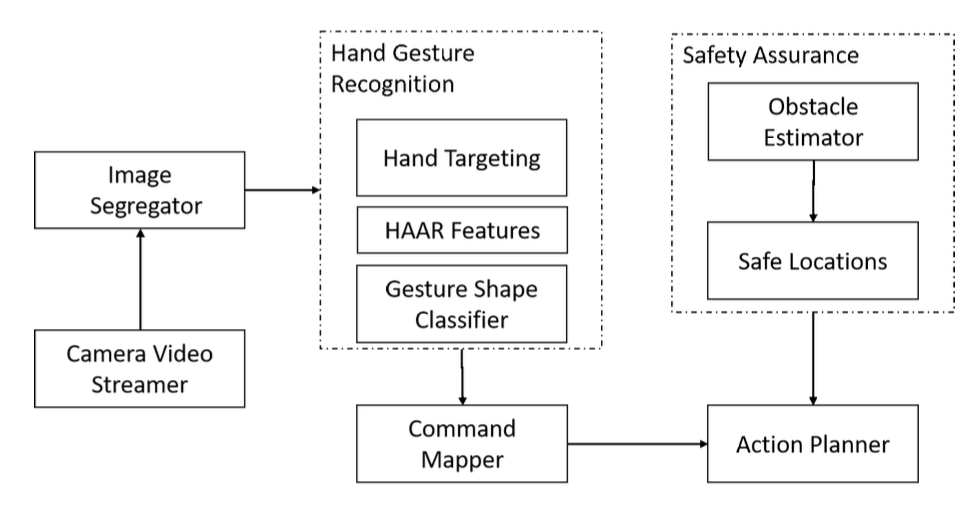
\includegraphics[width=0.8\textwidth]{Haar2.png}
    \caption{چارچوب کنترل پهپاد مبتنی بر ژست}
\end{figure}


\begin{figure}[h]
    \centering
    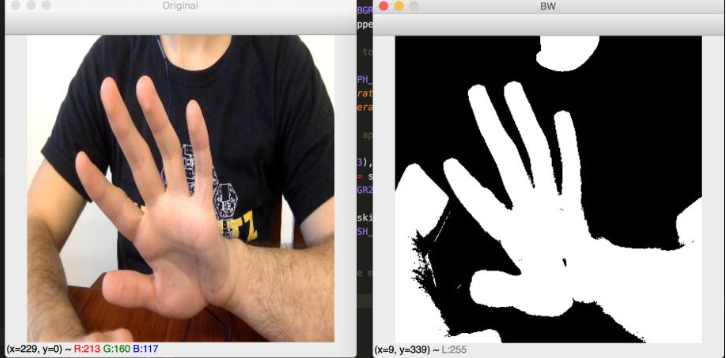
\includegraphics[width=0.5\textwidth]{Haar3.png}
    \caption{ ویژگی های \lr{Haar} برای استفاده از آستانه رنگ پوست برای تشخیص دست}
\end{figure}


در نهایت، این ویژگی‌ها به‌عنوان ورودی یک شبکه \lr{SVM} \LTRfootnote{Support Vector Machine} داده شده تا ژست دست تشخیص داده شود.

\subsubsection{نتیجه بدست آمده}
این پروژه دقت بالایی در تشخیص ژست دست و کنترل پرواز پهپاد دست می یابد. برای خروجی این پروژه ۵ حالت دست مدنظر قرار گرفته‌اند. 
دقت متوسط آن برابر 471.97 درصد است که عملکرد عالی را نشان می‌دهد. البته قابل ذکر است که این دقت در پس‌زمینه‌های بهم ریخته و همچنین در شرایط نوری مختلف بسیار متغیر است  زیرا همان‌طور که گفته‌شد ویژگی \lr{Haar} به سایه و رنگ‌های درون تصویر بسیار حساس است \cite{natarajan2018hand}.



\subsection{مقاله \lr{Hand Gesture Controlled Drones: An Open Source Library}}
در این پروژه نیز از ویژگی‌های \lr{Haar} استفاده شده تا بتوان ۹ حالت دست را شناسایی کرد. 

\subsubsection{روش‌شناسی}
در این مقاله نیز مانند پروژه قبل از استخراج ویژگی‌های \lr{Haar} استفاده شده. با این تفاوت که در مقاله قبل از معماری \lr{SVM} برای کلاس‌بندی ژست‌های دست استفاده شده است، در حالی که در این مقاله از شبکه \lr{ٰVGG-16} که به صورت لایه‌های کانولوشن است استفاده شده.

\begin{figure}[h]
    \centering
    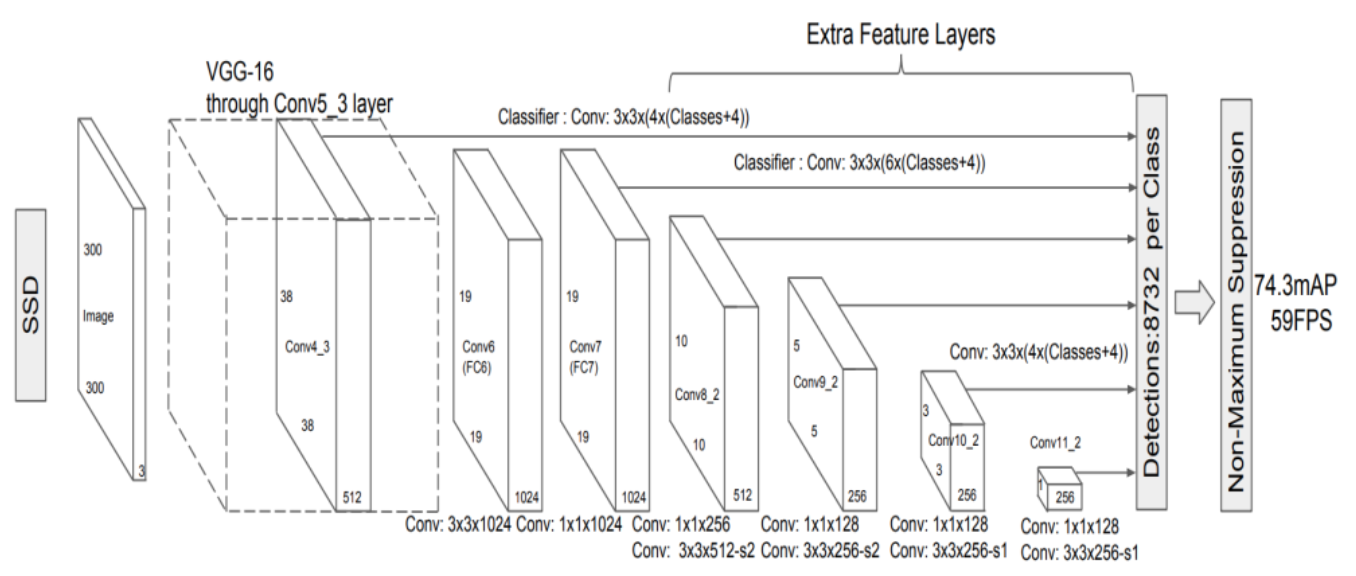
\includegraphics[width=0.8\textwidth]{VGG16.png}
    \caption{معماری \lr{VGG-16}}
\end{figure}


\subsubsection{نتیجه بدست آمده}
 در پروژه این پروژه ۹ حالت دست مدنظر قرار گرفته‌شده و دقت آن برابر ۳.۸۳ درصد است.
 که در بهترین حالت ممکن با پس‌زمینه‌ی مناسب بدست آمده و باید در نظر گرفت که دقت بالایی برای کنترل پهپاد به حساب نمی‌آید.



\subsection{مقاله \lr{Deep Learning Based Hand Gesture Recognition and UAV Flight Controls}}

\subsubsection{روش‌شناسی}
بدین صورت که در هر یک از فریم‌ها دریافت شده ویژگی‌های خاصی را استخراج می‌کند. از جمله این پارامترها زاویه انحراف، مختصات، قدرت گرفتن دست است که به صورت یک ماتریس ۴۵*۱۵ بدست می‌آید. در ادامه با ورود این پارمتر‌ها به صورت متوالی به شبکه و دریافت خروجی می‌تواند هدف حرکت کاربر را نشان دهد
\subsubsection{نتیجه}

\cite{hu2020deep}


\section{مقالات مربوط به ورودی تصویر دست}


\subsection{مقاله \lr{UAV-GESTURE: A Dataset for UAV Control and Gesture Recognition}}
این مقاله با هدف کنترل پهپاد یا خلبان خودکار با کمک حرکت دست پیاده‌سازی شده است. برای مثال حرکت چپ به راست دست نشان دهنده حرکت پهپاد به راست است. بدین ترتیب برای اجرای این برنامه شبکه \lr{P-CNN} طراحی شده است تا یتواند معنای عکس‌ها را تجربه کند.

\subsubsection{روش‌شناسی}
در این مقاله از شبکه‌‌ \lr{P-CNN} استفاده می‌شود. بدین‌صورت که در ابتدا موقعیت دست فرد با کمک جعبه مرزی \LTRfootnote{Bounding box} پیدا کرده، سپس عکس دست با فیلترهای مناسب وارد شبکه‌ی \lr{P-CNN} می‌شود تا بتوان ژست دست را پیش‌بینی کرد. در خروجی مدل ۱۳ نوع حرکت وجود دارد تا بتواند معنای آنها را پیش‌بینی کند. این حرکات برخلاف دیگر مقالات کل دست از شانه تا انگشتان و حرکات آنها شامل می‌شود. زیرا هدف اصلی آن دستور دادن به هواپیما‌های
 بزرگ بدون سرنشین در فررودگاه‌ها است. از آنجایی که دستان در تصاویر گرفته‌شده نسبتا کوچک‌اند، کیفیت تصاویر باید بالا باشد. از طرف دیگر از آنجایی که در این پروژه حرکات دست مدنظر است نه ژست آنها، توالی موقعیت و ژست دست‌هاست که اهمیت دارد. این توالی فریم‌ها سبب می‌شود تا مدل پیچیده و سنگینی داشته باشیم.

\subsubsection{نتیجه}
دقت مدل در بهترین حالت، با بهترین دیتاست ممکن برابر ۹.۹۱ درصد است که دقت بالایی برای اجرای پروژه است. اما به دلیل پیچیده و سنگین بودن مدل این پروژه یکی از بزرگ‌ترین اهداف پروژه که زمان واقعی بودن آن است دچار چالش می‌شود.\cite{perera2018uav}

% در این مقاله از شبکه‌‌های کانولوشن استفاده می‌شود. بدین صورت  که ابتدا یک شبکه موقعیت دست را استخراح می‌کند 



\section{مقالات مربوط به نقاط کلیدی دست}

\subsection{مقاله \lr{MediaPipe Hands: On-device Real-time Hand Tracking } و \lr{Applying Hand Gesture Recognition for User Guide Application Using MediaPipe}}
در این مقاله‌ها از کتابخانه \lr{MediaPipe} استفاده‌ شده‌است تا بتوان ۲۱ نقطه عطف دست را پیدا کرده و در پروژه‌های گوناگون از جمله پیدا کردن ژست دست و افکت‌های \lr{AR} استفاده کند. ما در پروژه خود از این کتابخانه استفاده می‌کنیم تا بتوانیم مدلی سبک و ساده پیاده کنیم.

\subsubsection{روش‌شناسی}
 در این مقاله به یررسی این کتابخانه پرداخته‌شده و ما از آن استفاده می‌کنیم تا بتوانیم مدلی برای پیش‌بینی ژست دست استفاده کنیم.
برای پیاده‌سازی این پروژه از دو شبکه کانولوشن استفاده شده است. شبکه اول که برای پیدا کردن کف دست در تصویر استفاده می‌شود و شبکه دوم که به عنوان ورودی موقعیت عکس دست پیدا شده را دریافت و مختصات ۲۱ تقطه عطف را موقعیت‌یابی می‌کند.


% \section{مقاله \lr{MediaPipe Hands: On-device Real-time Hand Tracking } و \lr{Applying Hand Gesture Recognition for User Guide Application Using MediaPipe}}
% در این مقاله از کتابخانه \lr{MediaPipe} استفاده‌ شده‌است. بدین صورت که ابتدا موقعیت دست را پیدا کرده، سپس مختصات ۲۱ تقطه عطف را موقعیت‌یابی می‌کند. در این مقاله به یررسی این کتابخانه پرداخته‌شده و ما از آن استفاده می‌کنیم تا بتوانیم مدلی برای پیش‌بینی ژست دست استفاده کنیم که ساده و سبک‌ باشد.

% \subsection{روش‌شناسی}
% برای پیاده‌سازی این پروژه از دو شبکه کانولوشن استفاده شده است. شبکه اول که برای پیدا کردن کف دست در تصویر استفاده می‌شود

% \subsection{روش‌شناسی}
% برای پیاده‌سازی این پروژه از دو شبکه کانولوشن استفاده شده است. شبکه اول که برای پیدا کردن کف دست در تصویر استفاده می‌شود


\subsubsection{نتیجه}
مدل‌های طراحی شده در این مقالات برای تشخیص نقاط عطف دست از دقت ۷.۹۵ درصد برخوردار هستند که دقت بسیار بالایی محاسبه می‌شود. همچنین این مدل به نور و تصویر پس‌زمینه وابسته نیست و دقت متوسط آن در زمینه‌های مختلف اندازه‌گیری شده لذا مدل را کاربردی‌ و مورد پسندتر می‌کند\cite{zhang2020mediapipe} \cite{harris2021applying}.



\section{مقالات مربوط به اجرای مدل‌های بینایی کامپیوتر روی پهپاد}


\section{جمع‌بندی}


در تمام مقالات بررسی شده، پروژه‌ها به گونه‌ای پیاده‌سازی شده‌اند تا حرکات را به طوری کلاس‌بندی کنند که در خروجی حتما یکی از ژست‌های درنظر گرفته‌شده انتخاب شود. لذا زمانی که دست در حالتی غیر از آنها قرار دارد، مدل طراحی شده حتما یکی از ژست‌هایی را که به آن شبیه‌تر است را انتخاب می‌کند که این امر می‌تواند برای پیاده‌سازی روی پهپاد واقعی مشکل‌زا باشد و حتی هزینه مالی به ارمفان آورد.
